\chapter{Projet Détection et reconnaissance de véhicules militaires sur des images et vidéos (DetReco)}
\label{chap:3}
\sloppy

\section{Définition}

Avant de commencer le travail effectué, nous allons rappeler les éléments sur lesquels porte le projet.
\subsection{Détection}
La détection est la capacité à distinguer un objet du fond. Le critère d'évaluation est la distance maximale à laquelle se perçoit l'objet. La détection à longue distance ne permet pas la reconnaissance de la cible, seulement d'en détecter la présence.

Pour entraîner un algorithme de détection, il faut fournir des images présentant l'objet cible à la distance maximale visée. On définit la taille des cibles pixels minimum nécessaires pour la détection. Ainsi, pour la détection, il faudra au minimum \textbf{4x8 pixels}.


\subsection{Reconnaissance}

La reconnaissance est la capacité à classifier un objet dans une catégorie. Le critère d'évaluation est la distance maximale à laquelle l'objet peut être reconnu correctement. La taille minimale nécessaire pour la reconnaissance est d'au moins \textbf{20x40 pixels}.

La reconnaissance nécessite la définition d'une classification des véhicules cibles. Plusieurs pistes ont été proposées par la DGA TT : classification des véhicules par catégories (véhicules blindés, moyens anti-char, artillerie sol-sol, etc.). La difficulté pour l'établissement d'une classification vient de l'ambiguïté des classes assignables à certaines catégories. Notamment, un véhicule d'une même catégorie peut avoir différentes fonctions, raison pour laquelle une classification par catégorie élargie est à privilégier.


\subsection{Identification}

L'identification est la capacité à identifier précisément un objet cible. L'identification par enregistrement s'appuie sur des clés d'identification spécifiques pour chaque matériel. Dans le cadre de ce projet, l'identification est laissée hors périmètre.


\section{Modèle d'entraînement}

Les algorithmes de l’état de l’art proposés dans le cadre de ce projet sont :

\begin{itemize}
    \item Pour la détection : \textbf{YoloVx} \cite{jocher2023yolo}, \textbf{Faster RCNN} \cite{ren2016faster}, \textbf{Grounding DINO} \cite{liu2023grounding}.
    \item Pour le suivi d’objets (tracking) : \textbf{DeepSort} \cite{wojke2017simple}, \textbf{ByteTrack} \cite{zhang2022bytetrack}.
\end{itemize}

Dans le cadre de ce projet, nous avons implémenté un algorithme qui s’appuie sur le modèle \textbf{YOLOv8} pour la détection et l’algorithme \textbf{DeepOCsort} \cite{maggioolino2023deep} pour le tracking de véhicules.\\

De base, nous utilisons le modèle \textbf{yolov8m.pt} (medium), qui offre un bon compromis entre taille et vitesse, mais d'autres modèles que nous utiliserons pour l'expérience, sont disponibles auprès \textit{d'ultralytics}.

\begin{table}[H]
    \centering
    \begin{tabular}{|p{2cm}|p{2cm}|p{1.7cm}|p{2.4cm}|p{2.4cm}|p{1.7cm}|p{1.7cm}|}
        \hline
        \textbf{Model}   & \textbf{Size (pixels)} & \textbf{mAP\textsuperscript{val} 50-95} & \textbf{Speed CPU ONNX (ms)} & \textbf{Speed A100 TensorRT (ms)} & \textbf{Params (M)} & \textbf{FLOPs (B)} \\ \hline
        \textit{YOLOv8n} & 640                    & 37.3                                    & 80.4                         & 0.99                              & 3.2                 & 8.7                \\ \hline
        \textit{YOLOv8s} & 640                    & 44.9                                    & 128.4                        & 1.20                              & 11.2                & 28.6               \\ \hline
        \textit{YOLOv8m} & 640                    & 50.2                                    & 234.7                        & 1.83                              & 25.9                & 78.9               \\ \hline
        \textit{YOLOv8l} & 640                    & 52.9                                    & 375.2                        & 2.39                              & 43.7                & 165.2              \\ \hline
        \textit{YOLOv8x} & 640                    & 53.9                                    & 479.1                        & 3.53                              & 68.2                & 257.8              \\ \hline
    \end{tabular}
    \caption{Comparaison des modèles YOLOv8 \cite{jocher2023yolo}}
    \label{tab:yolov8_comparaison}
\end{table}




\section{Constitution d’une base de données d’entraînement}

Cette partie du travail a pour objectif la création d'une base de données d’images permettant l’entraînement d’un algorithme de détection et reconnaissance de véhicules militaires à l'état de l'art.

Il s’agit d’identifier un algorithme cible de l’état de l’art pouvant servir de référence pour l’évaluation de la qualité du jeu de données, et d’identifier les caractéristiques du jeu de données pertinentes pour la qualité du modèle entraîné.
En effet, les modèles de deep-learning visés par la convention DetReco sont fortement sensibles aux jeux de données utilisés pour les entraîner.
Les caractéristiques qui peuvent jouer sur la qualité du modèle entraîné sont :

\begin{itemize}
    \item dimensions et résolutions des images,
    \item luminosité,
    \item dimensions et nombre des objets cibles à détecter dans l’image (gros plan, arrière plan, etc.),
    \item visibilité de l’objet cible (occulté, ou bien peu visible en raison des conditions de la mise en scène telles que brouillard, pluie, neige, fumée, obstacles, etc.),
    \item diversité et représentativité des classes.
\end{itemize}

Un algorithme qui n’aurait été entraîné que sur un sous-ensemble des données possibles serait inapte à détecter les véhicules dans des conditions qu’il ne connaît pas.
Ainsi,pour pouvoir détecter des objets dans des conditions de terrain réelles, il est nécessaire de constituer un jeu de données au plus proche possible de ces conditions



\subsection{Définition des classes}

Afin de développer un modèle capable de faire la différence entre différents types de véhicules militaires, nous allons classifier les véhicules.

La définition d’une classification pose problème en raison de l’ambiguïté des véhicules pouvant se retrouver dans plusieurs classes.
Une première classification a été proposée pour regrouper les véhicules dans des catégories larges :

Nous utiliserons 4 classes :

\begin{itemize}
    \item Armoured Fighting Vehicle \textbf{(AFV) :} véhicules blindés de combat. (Figure \ref{fig:afv})
    \item Armoured Personnel Carrier \textbf{(APC) :} véhicules blindés pour transport des troupes. (Figure \ref{fig:apc})
    \item Military Engineering Vehicle \textbf{(MEV) :} véhicules conçu pour les travaux de construction. (Figure \ref{fig:mev})
    \item Light armoured vehicle \textbf{(LAV) :} véhicules blindés légers. (Figure \ref{fig:lav})
\end{itemize}
Cette classification pourra être amendée en fonction des résultats obtenus par l’algorithme de détection et de l’expertise de la DGA TT.


\begin{figure}[H]
    \centering
    \begin{subfigure}[b]{0.45\textwidth}
        \centering
        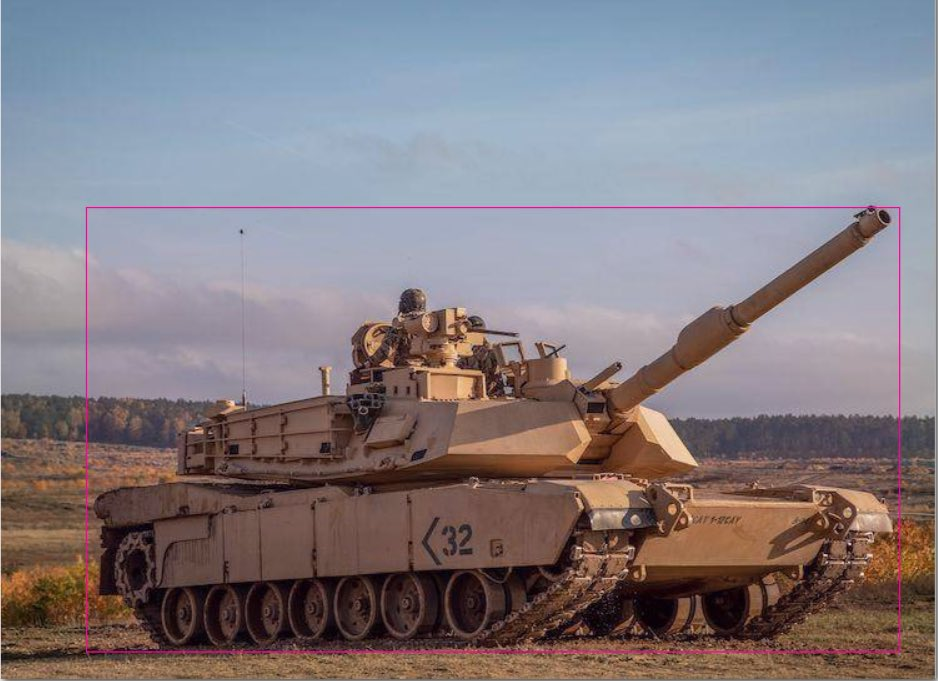
\includegraphics[width=\textwidth]{./images/afv.png}
        \caption{\textbf{AFV} - char M1 Abrams}
        \label{fig:afv}
    \end{subfigure}
    \hfill
    \begin{subfigure}[b]{0.45\textwidth}
        \centering
        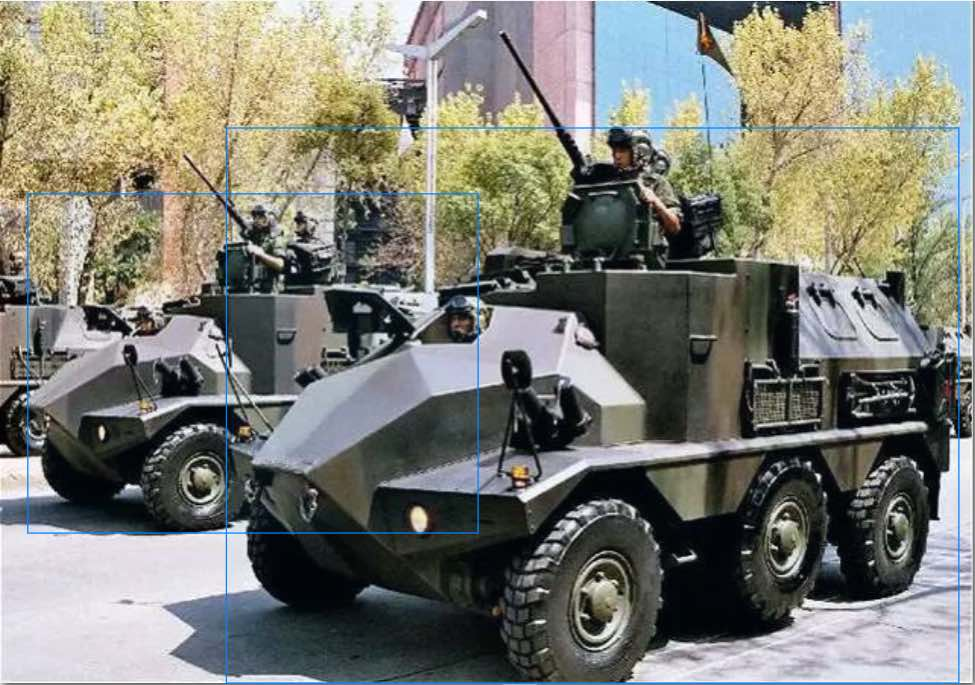
\includegraphics[width=\textwidth]{./images/apc.png}
        \caption{\textbf{APC} - Panhard VCR}
        \label{fig:apc}
    \end{subfigure}
    \vskip\baselineskip
    \begin{subfigure}[b]{0.45\textwidth}
        \centering
        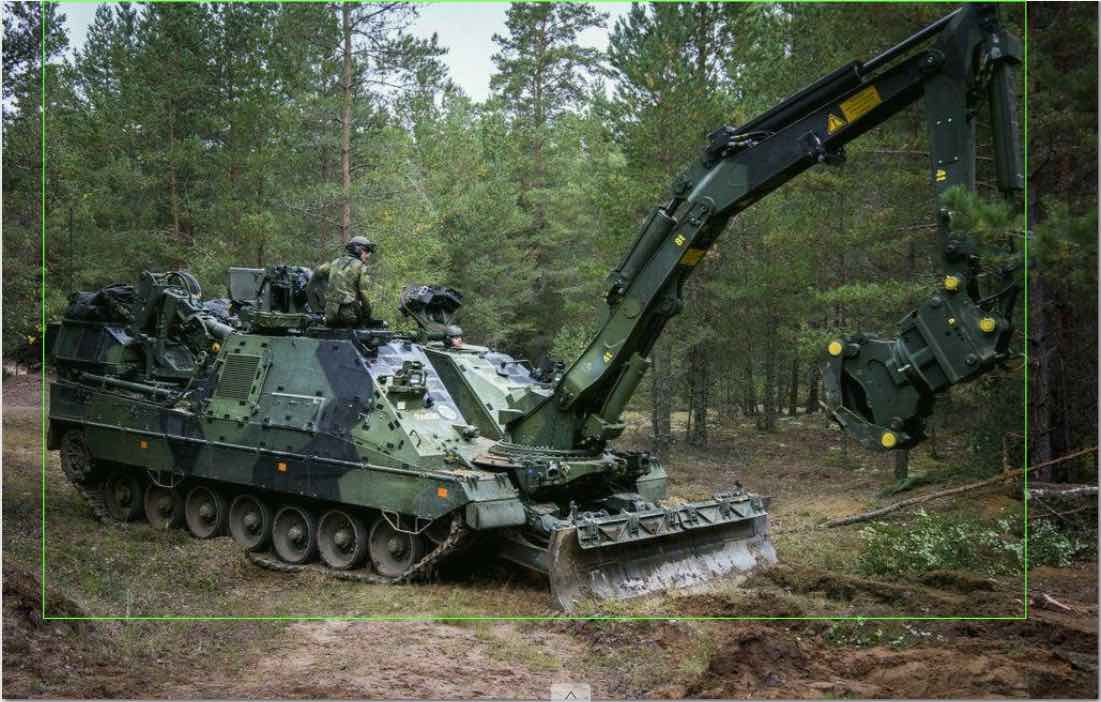
\includegraphics[width=\textwidth]{./images/mev.png}
        \caption{\textbf{MEV} - Kodiak Wisent}
        \label{fig:mev}
    \end{subfigure}
    \hfill
    \begin{subfigure}[b]{0.45\textwidth}
        \centering
        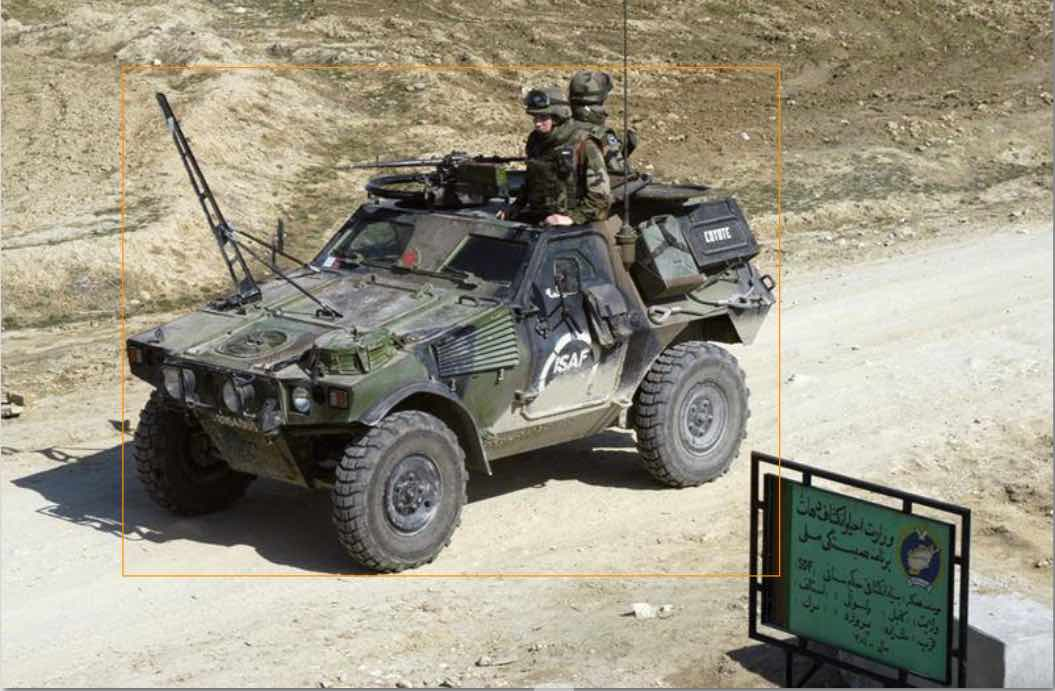
\includegraphics[width=\textwidth]{./images/lav.png}
        \caption{\textbf{LAV} - Panhard VBL}
        \label{fig:lav}
    \end{subfigure}
    \caption{Exemples de véhicules militaires}
    \label{fig:military-vehicles}
\end{figure}


\subsection{Jeu de données d’entraînement}

Nous avons identifié des sources de jeux de données et images  utilisés pour l’entraînement d’algorithmes de visualisation, et des images open source sur Internet.

Nous décrivons dans cette section les jeux de données identifiés et utilisés pour l’entraînement de l’algorithme YoloV8 de détection.

\subsubsection{Open Images v7}

Open Images \cite{openimages2024} est un jeu de données d’environ 9 million d’images annotées, avec notamment 16 million d’annotations bounding boxes pour 600 classes.
Parmi ces classes, une classe Tank contient \textbf{1248 images annotées de véhicules militaires}.

\begin{figure}[H]
    \center
    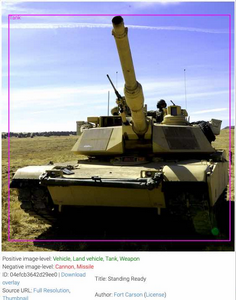
\includegraphics[width=0.5\textwidth]{./images/char-leclerc-openv7.png}
    \caption[Image annotée d’un char]{Image annotée d’un char, extraite du jeu de données Open Images v7.}\label{fig:image-annotée-char}
\end{figure}

\subsubsection{ImageNet}

Le jeu de données ImageNet, créé pour le challenge de détection ILSVRC2012 \cite{imagenet2012}, a été au centre des avancées récentes dans le domaine de la reconnaissance automatique d’objets dans des images par deep-learning.
Ce jeu de données sert aujourd’hui de jeu de données standard pour l’entraînement d’algorithmes de transfert learning.
Il contient plus de 14 million d’images annotées, divisées en 21841 classes.

Parmi ces 21841 classes, plusieurs peuvent contenir des images pertinentes pour la reconnaissance de véhicules militaires. Par exemple, les classes

\begin{itemize}
    \item n02739889 (armored car, armoured car),
    \item n02740061 (armored car, armoured car),
    \item n02740300 (armored personnel carrier, armoured personnel carrier, APC),
    \item n02740533 (armored vehicle, armoured vehicle),
    \item n04389033 (tank, army tank, armored combat vehicle, armoured combat vehicle).
\end{itemize}

Néanmoins, parmi celles-ci seules les images de la classe n04389033 (tank, army tank, armored combat vehicle, armoured combat vehicle) contiennent des annotations pour la détection d’objets.
Cette classe contient \textbf{378 images annotées de véhicules militaires}.

\subsubsection{Roboflow}

Nous disposons désormais de 1624 images annotées de tank, mais cela reste insuffisant pour un entraînement optimal du modèle. Pour obtenir encore plus d'images d'entraînement, nous avons charger un autre dataset annotées de véhicules militaires, mis à disposition par \textit{Tuomo Hiippala du Digital Geography Lab}.\cite{roboflow2024}
Ce jeu de données contient \textbf{1042 images} dont 89 images négatives avec 10 classes (bm-21, t-80, t-64, t-72, bmp-1, bmp-2, bmd-2, btr-70, btr-80 et mt-lb) que nous avons par la suite mapper en AFV (tank).


\subsubsection{Données disponibles librement}

Une recherche d’images sur Internet permet de trouver aisément des exemples pouvant servir à l’entraînement d’un algorithme de détection de véhicules. (Google)
Plusieurs facteurs sont cependant à prendre en compte.


\begin{itemize}
    \item Premièrement, les images que l’on peut trouver ne sont pas annotées, et demandent donc un travail supplémentaire d’annotation manuelle.
          \begin{figure}[H]
              \center
              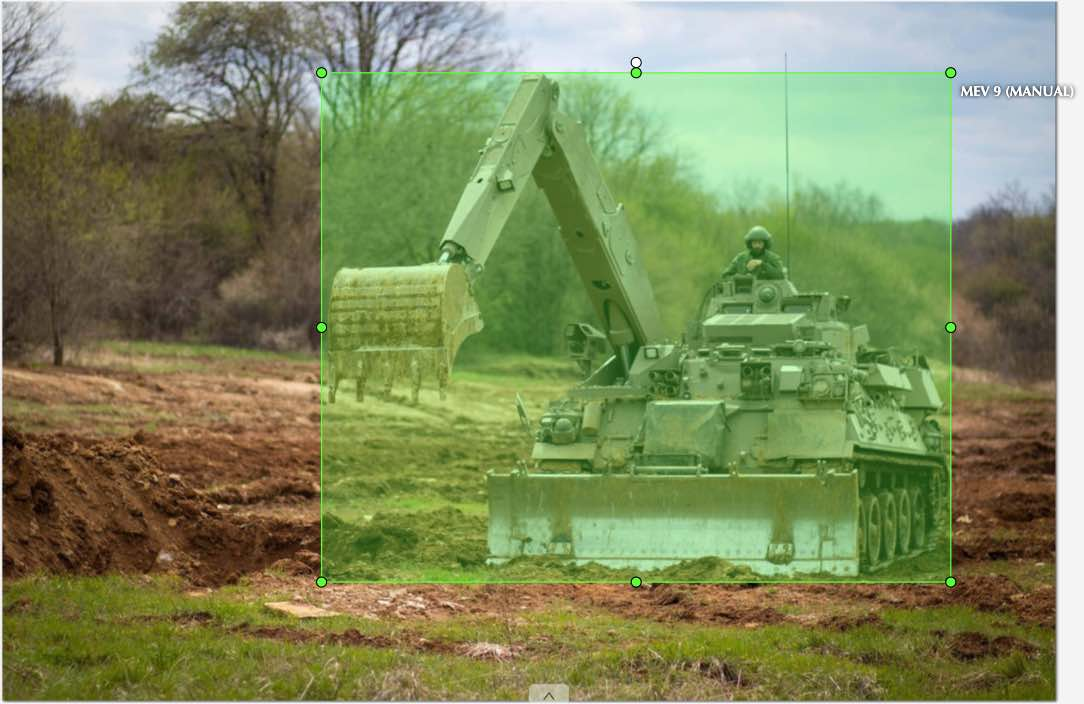
\includegraphics[width=0.6\textwidth]{./images/anotation-manuelle.png}
              \caption{Annotation manuelle d’une image d’engin blindé du génie.}\label{fig:anotation-manuelle}
          \end{figure}
    \item Deuxièmement, ces images servent principalement à répondre aux attentes des utilisateurs d’un moteur de recherche, et ne correspondent pas nécessairement aux critères attendus pour l’entraînement d’un algorithme de détection d’objets.
          Ainsi, une recherche d’images de char Leclerc donnera des résultats qui présentent l’objet en gros plan, clairement identifiable.
          Il est difficile d’obtenir des images qui présentent l’objet « en situation réelle de combat », ce qui limitera la qualité du modèle entraîné.
\end{itemize}

Nous avons tout de même pu constituer, à partir d’une recherche limitée pour certains modèles de véhicules militaires, un premier corpus composé de \textbf{669 images}. Nous avons annoté manuellement ces 669 images avec quatre classes.\\


\subsubsection{Etapes de collecte}

Nous avons reparti la collecte en deux grandes étapes:\\

\indent \textbf{Prepare-01 :} Nous commençons par créer un jeu de données d'entraînement à partir des données disponibles librement sur Internet. (ImageNet, OpenImages, Roboflow).

\noindent Pour cette première étape, nous avons collecté \textbf{2666 images} de véhicules militaires dont \textbf{2577 images positives} et \textbf{89 images négatives}.
A cette étape, nous avons travaillé avec une classe \textbf{tank}.\\


\textbf{Prepare-02 :} Nous utilisons également des outils de scraping pour collecter davantage d'images de véhicules militaires à partir d'images Google.

\noindent Nous avons collectés 669 images de plus, ce qui nous fait un total de \textbf{3335 images de véhicules}. (Figure \ref{fig:fiftyone-dataset})

Ce nombre d'images nous permet de définir quatre grandes classes (AFV, APC, MEV et LAV) de véhicules militaires que notre modèle peut ensuite discriminer.


\begin{figure}[H]
    \center
    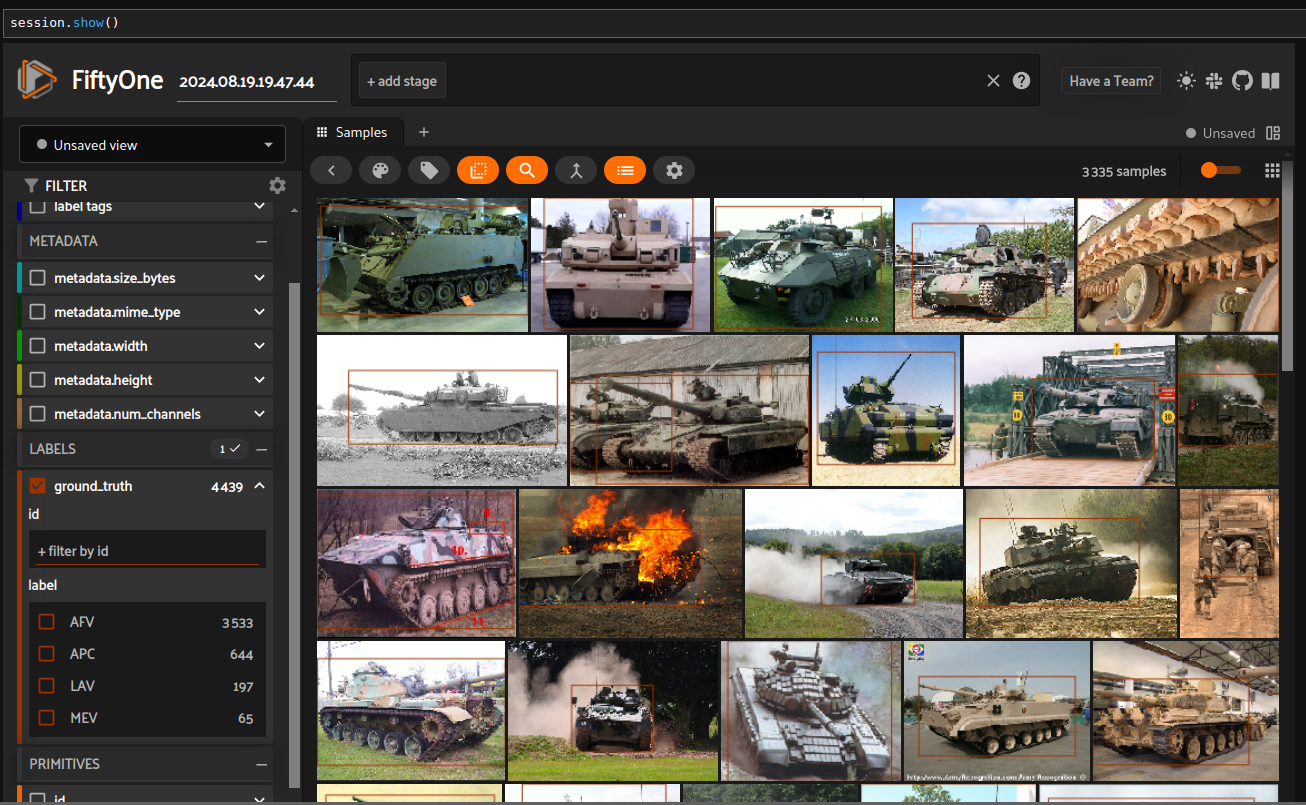
\includegraphics[width=0.8\textwidth]{./images/fiftyone-dataset.png}
    \caption[Fiftyone dataset]{FiftyOne - Jeu de données (3335 images)}\label{fig:fiftyone-dataset}
\end{figure}


\section{Résultats des premiers entraînements}

A ce niveau de l'expérience, la collecte des données du dataset d'entraînement c'est faite en deux grandes étapes (Prepare-01 et Prepare-02).
Nous allons présenter les résultats d'entraînement avec images positives et négatives sur les différentes tailles du modèles YoloV8.
Les images positives sont celles qui contiennent un ou plusieurs des objets définis (i.e. Tank, Camion militaire, Char militaire, ...).
Les images négatives sont celles qui contiennent autre chose que les objets définis.\\

La précision (\textbf{mAP : Mean Average Precision}) de notre modèle sera relevée à la fin de chaque entraînement afin de suivre son évolution.

\begin{equation}
    \mathrm{mAP} = \frac{1}{N} \sum_{i=1}^{N} \mathrm{AP}_i
\end{equation}

\begin{itemize}
    \item \textbf{N} : Représente le nombre total de classes dans le dataset.
    \item \textbf{AP$_i$} : Représente l'Average Precision (Précision Moyenne) pour la $i$-ème classe.
    \item \textbf{mAP} : Représente la moyenne des précisions moyennes sur toutes les classes.
\end{itemize}



\subsection*{Prepare-01: ImageNet, OpenImages, Roboflow (2666 images)}

A cette étape, le modèle détecte uniquement une classe 'tank', donc la mAP sera une moyenne de toutes les images.

Nous avons essayé plusieurs scénarios sur l’algorithme en changeant le paramètres \textit{Epoch} (époques: passe complète à travers toutes les instances de dataset d'entraînement.) et la taille du modèles.


\begin{itemize}
    \item \textbf{yolov8m :}
          \begin{itemize}
              \item \textbf{Avec images non annotées :}
                    \begin{itemize}
                        \item Epoch = 60 $\Rightarrow$ mAP = 0.660601
                        \item Epoch = 80 $\Rightarrow$ mAP = 0.6548
                        \item Epoch = 100 $\Rightarrow$ mAP = 0.6476
                    \end{itemize}
              \item \textbf{Sans images non annotées :}
                    \begin{itemize}
                        \item Epoch = 60 $\Rightarrow$ mAP = 0.71369
                        \item Epoch = 70 $\Rightarrow$ mAP = 0.692007695
                        \item Epoch = 80 $\Rightarrow$ mAP = 0.70
                        \item Epoch = 100 $\Rightarrow$ mAP = 0.70
                    \end{itemize}
          \end{itemize}

    \item \textbf{yolov8l :}
          \begin{itemize}
              \item \textbf{Avec images non annotées :}
                    \begin{itemize}
                        \item Epoch = 60 $\Rightarrow$ mAP = 0.6512
                        \item Epoch = 80 $\Rightarrow$ mAP = 0.6491
                        \item Epoch = 100 $\Rightarrow$ mAP = 0.6384
                    \end{itemize}
          \end{itemize}

    \item \textbf{yolov8x :}
          \begin{itemize}
              \item \textbf{Avec images non annotées :}
                    \begin{itemize}
                        \item Epoch = 60 $\Rightarrow$ mAP = 0.6518
                        \item Epoch = 80 $\Rightarrow$ mAP = 0.6535
                        \item Epoch = 100 $\Rightarrow$ mAP = 0.6308
                    \end{itemize}
          \end{itemize}
\end{itemize}


Au vu de ces résultats, nous nous sommes rendu compte que la taille du modèle n'influence pas les résultats. Nous allons donc uniquement travailler avec la taille medium du modèle YoloV8.
Nous allons également utiliser des datasets contenant des images annotées.


\subsection*{Prepare-02: ImageNet, OpenImages, Roboflow and Google  (3335 images)}

A cette étape, nous avons entraîné le modèle a détecter les 04 classes (AFV, APC, MEV, LAV).
La moyenne mAP tient donc compte de ces 04 classes, mais nous allons aussi fournir la moyenne de chacune des classes.

\begin{itemize}
    \item \textbf{yolov8m :}
          \begin{itemize}
              \item Epoch = 60 $\Rightarrow$ mAP = 0.6609276140054803
          \end{itemize}
\end{itemize}

\begin{figure}[H]
    \center
    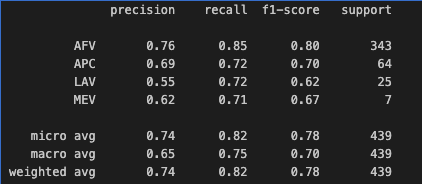
\includegraphics[width=0.6\textwidth]{./images/map-train.png}
    \caption[mAP des 04 classes]{mAP des 04 classes}\label{fig:map-train}
\end{figure}



\section{Tracking}

Après avoir entraîné notre model avec notre jeu de donnée, nous utilisons le meilleur model (\textbf{best.pt}) obtenu pendant l'entraînement et un tracker (\textbf{botsort.yaml}) pour tracker les objets dans les vidéos.


\begin{figure}[H]
    \center
    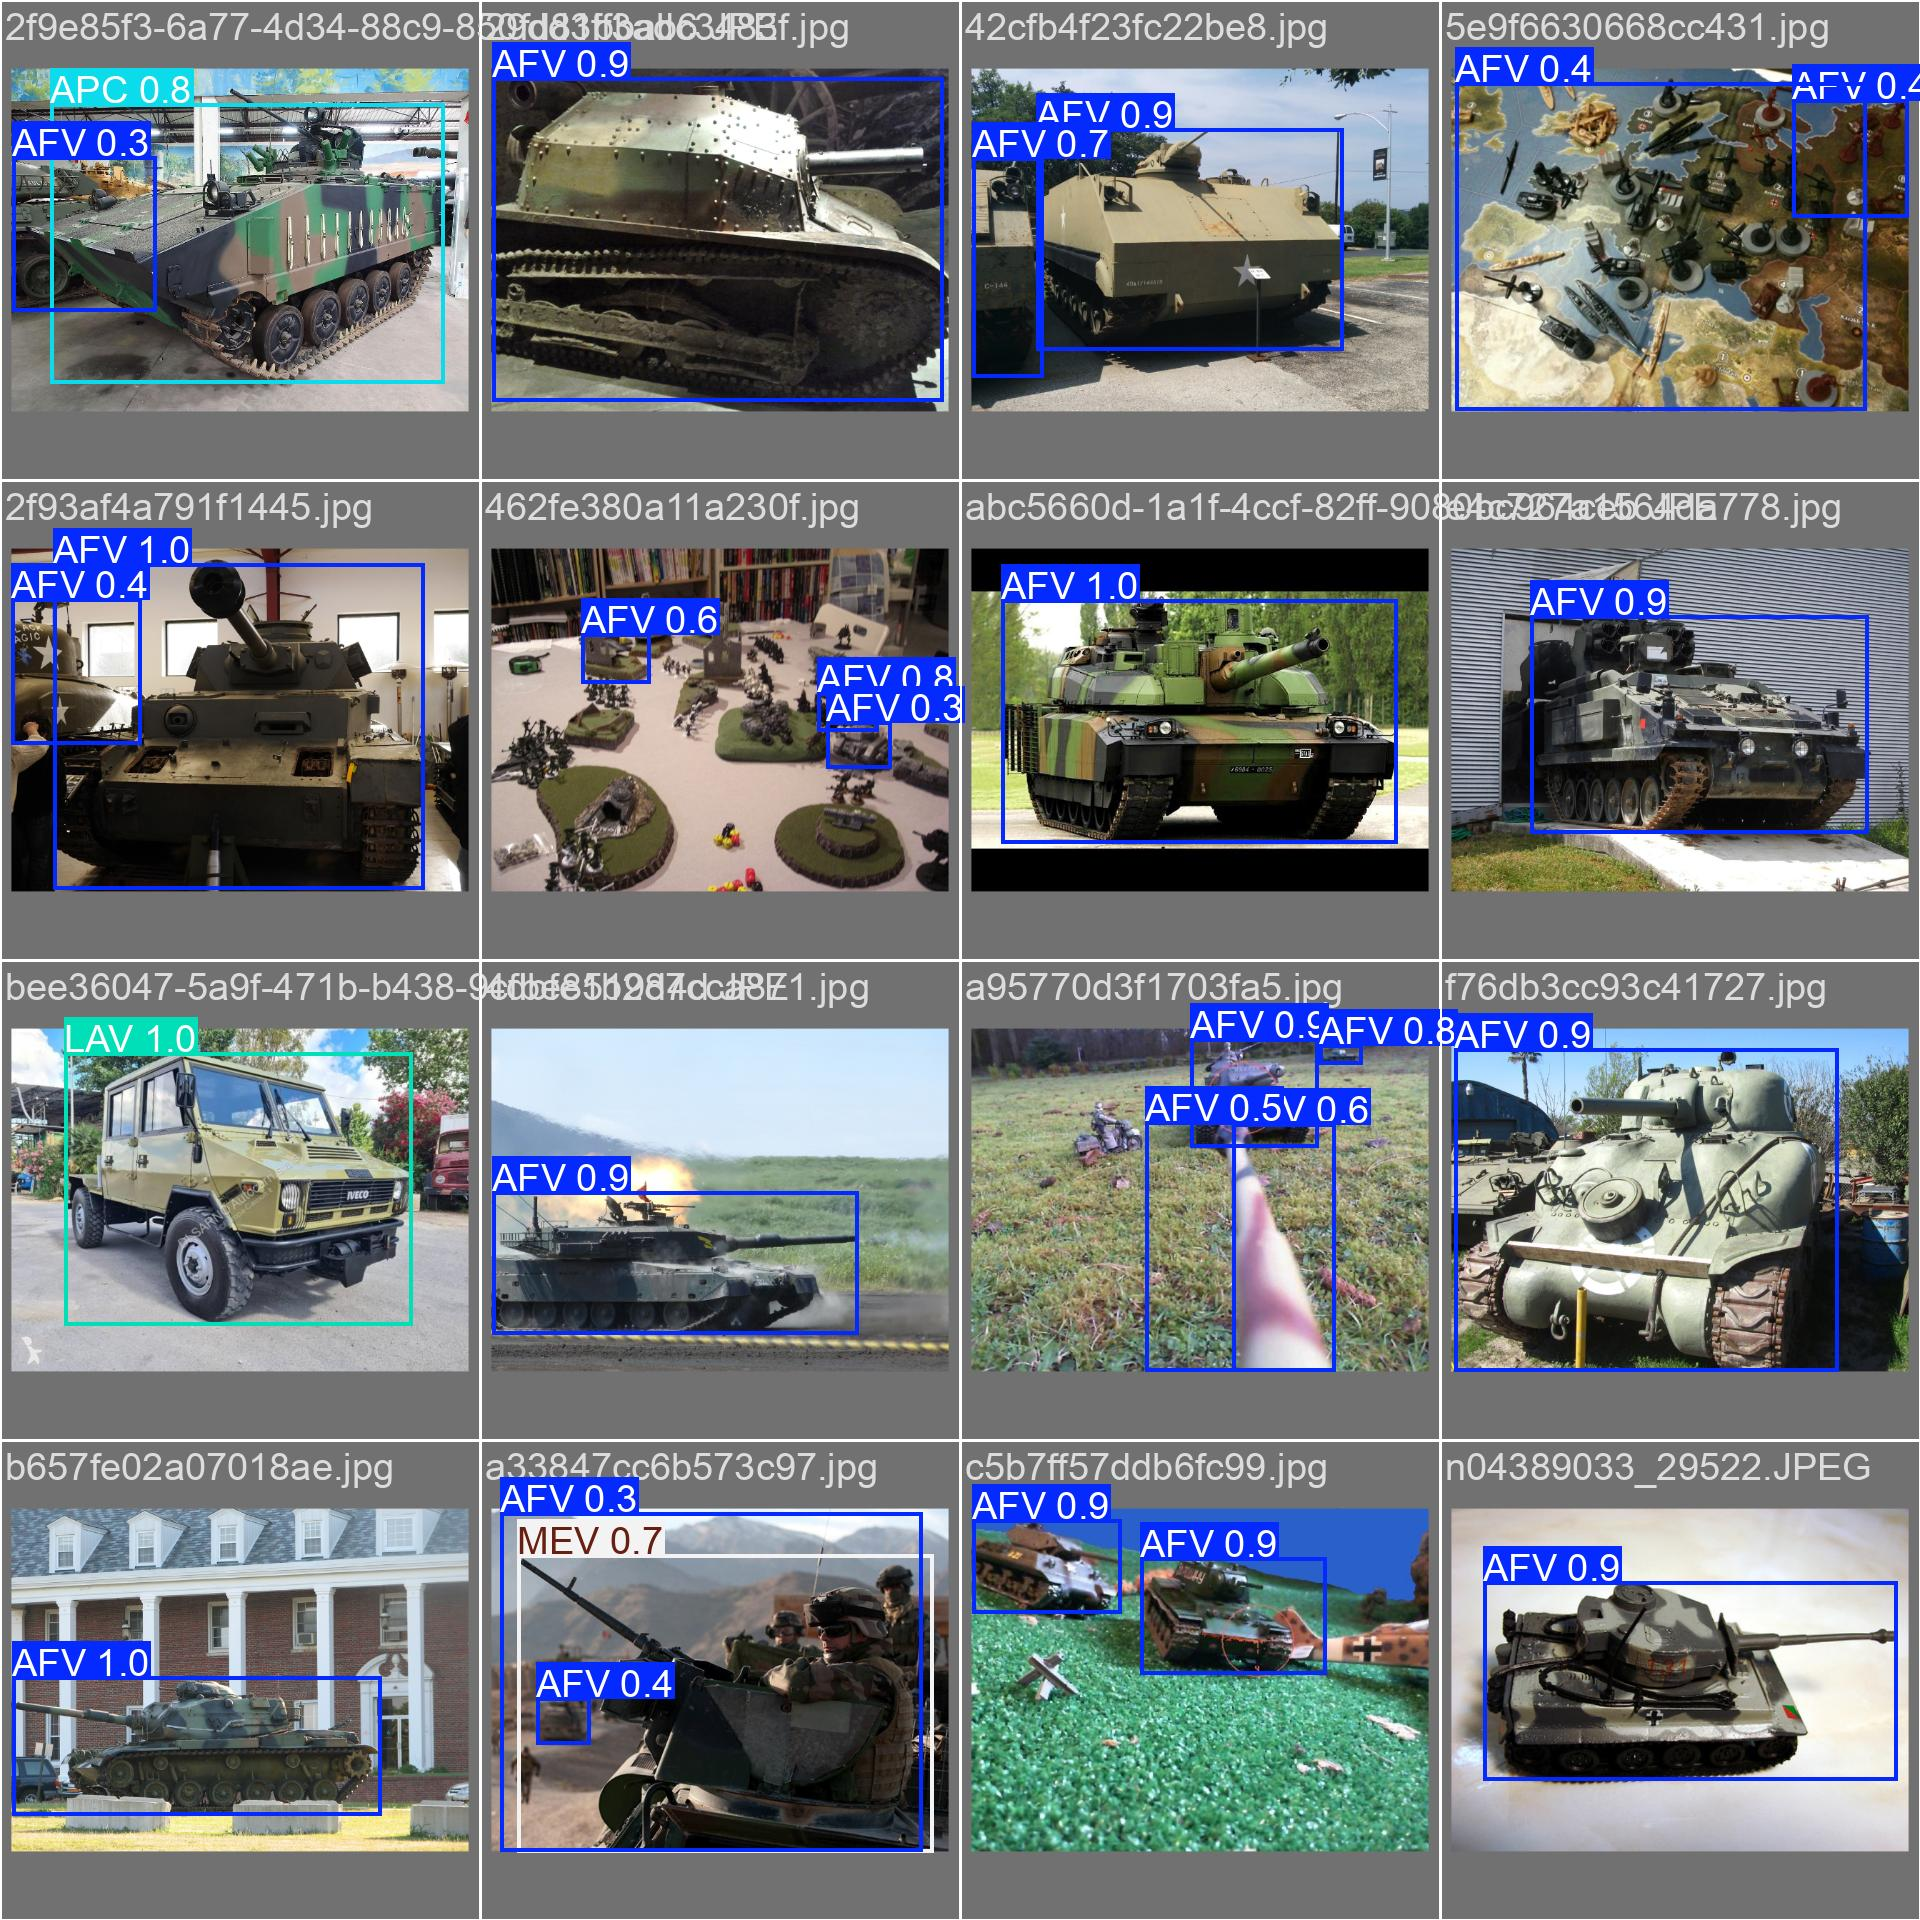
\includegraphics[width=0.6\textwidth]{./images/track2_val.jpg}
    \caption[Détection et reconnaissance avec taux de précision]{Détection et reconnaissance avec taux de précision}\label{fig:track2_val}
\end{figure}


\section{Augmentation des données}

\subsection{Images transformées}

Nous avons utilisé des méthodes d'augmentation des données afin d'améliorer la capacité du modèle à reconnaître des véhicules même lorsqu'ils sont éloignés ou partiellement masqués. Les méthodes utilisées incluent :

\begin{itemize}
    \item Une transformation \textbf{scale} pour dézoomer l'image et donner l'impression que le véhicule est vu de loin.
    \item Une transformation \textbf{XYMasking} pour masquer des bandes horizontales ou verticales, simulant un véhicule caché par un obstacle.
    \item Une transformation de type \textbf{Météo} pour donner l'impression qu'il y a de la neige, de la pluie ou du brouillard sur l'image.
\end{itemize}


\begin{figure}[H]
    \centering
    \begin{subfigure}[b]{0.45\textwidth}
        \centering
        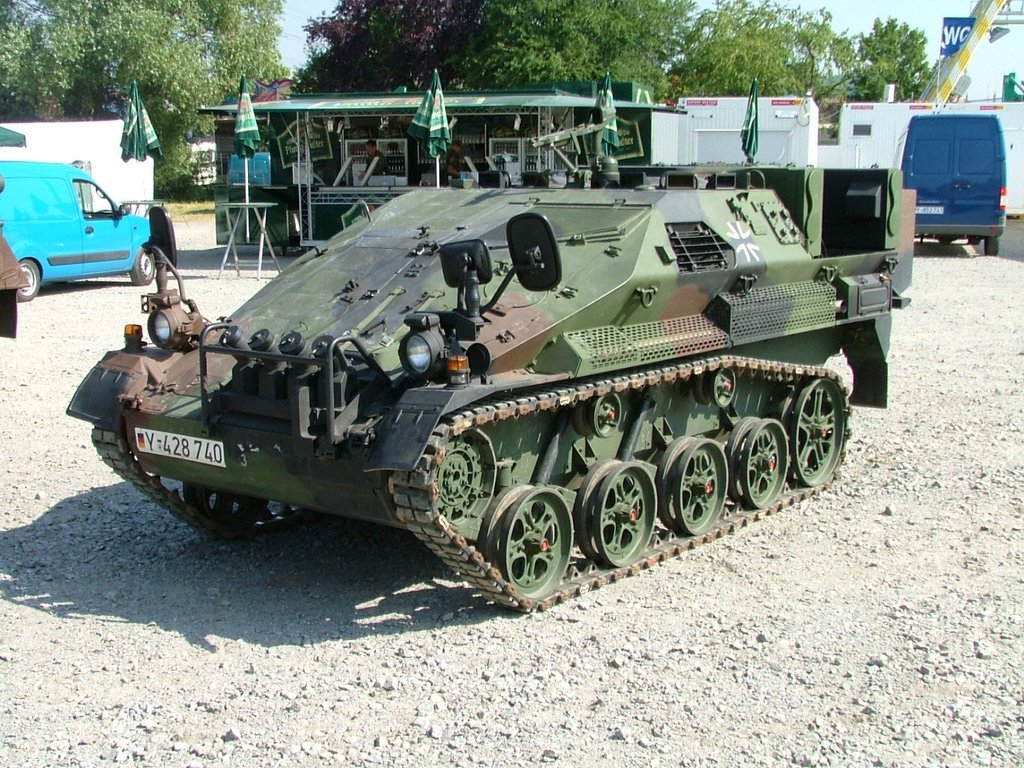
\includegraphics[width=\textwidth]{./images/original-image.jpg}
        \caption{Image originale}
        \label{fig:original-image}
    \end{subfigure}
    \hfill
    \begin{subfigure}[b]{0.45\textwidth}
        \centering
        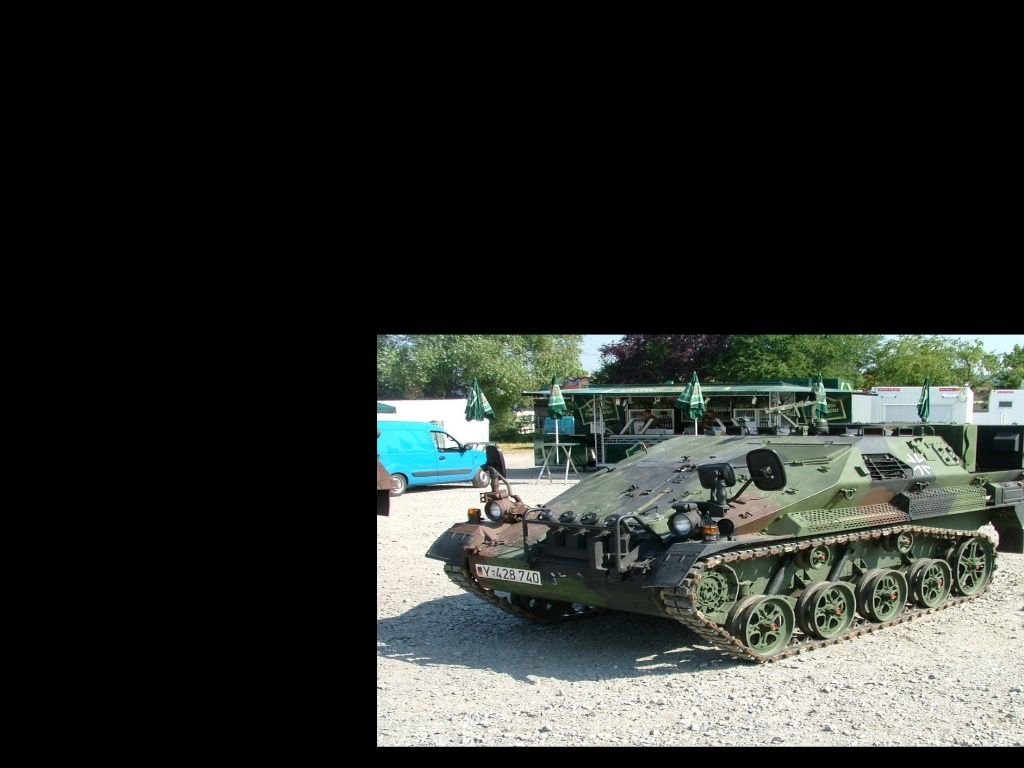
\includegraphics[width=\textwidth]{./images/scale_transformed.jpg}
        \caption{Effet zoom}
        \label{fig:scale_transformed}
    \end{subfigure}
    \vskip\baselineskip
    \begin{subfigure}[b]{0.45\textwidth}
        \centering
        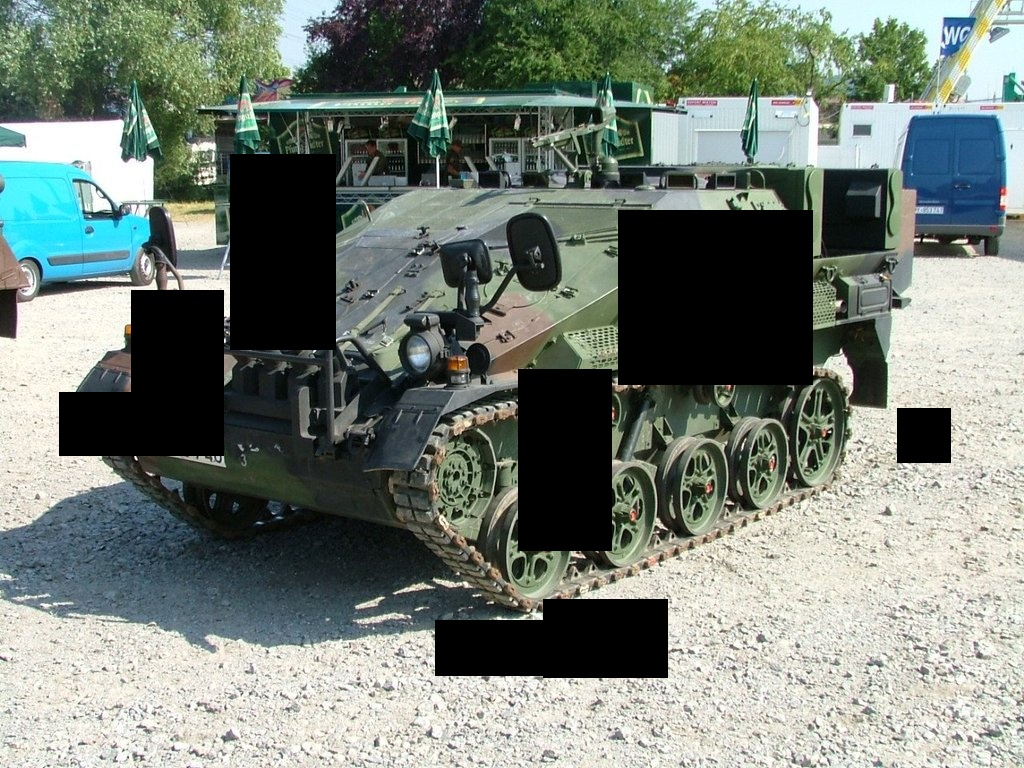
\includegraphics[width=\textwidth]{./images/xymasking.jpg}
        \caption{XYMasking}
        \label{fig:xymasking}
    \end{subfigure}
    \hfill
    \begin{subfigure}[b]{0.45\textwidth}
        \centering
        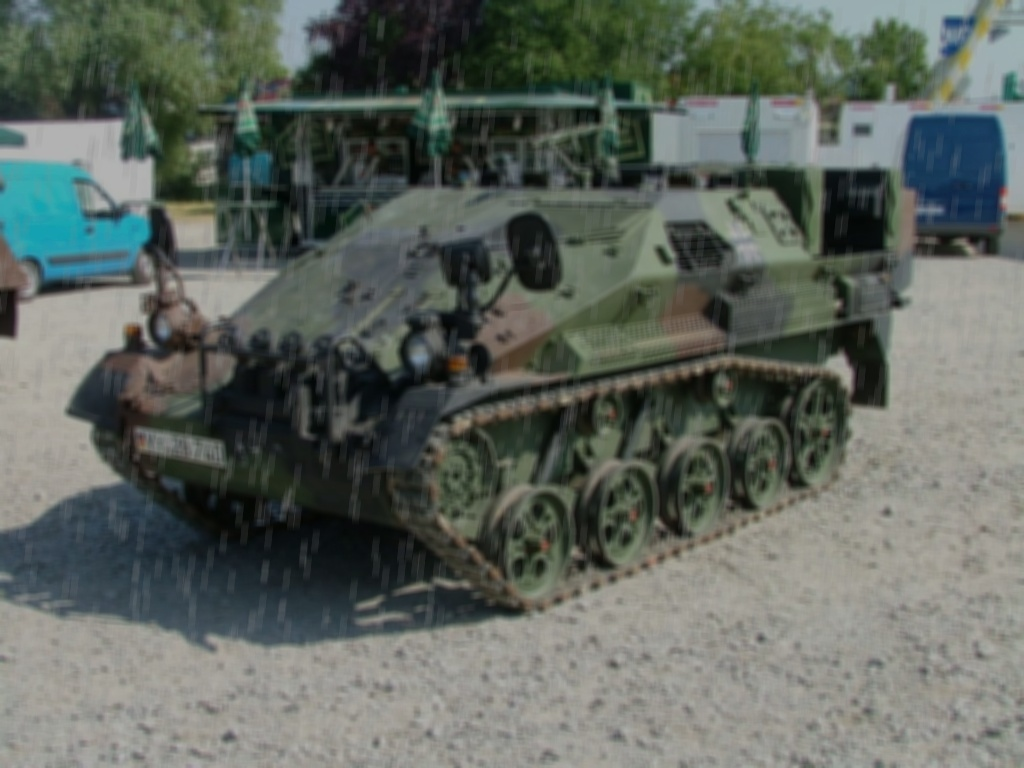
\includegraphics[width=\textwidth]{./images/weather_effect.jpg}
        \caption{Météo (pluie)}
        \label{fig:meteo}
    \end{subfigure}
    \caption{Exemples transformation d'images de véhicules militaires}
    \label{fig:military-vehicles}
\end{figure}




\noindent Les étapes spécifiques suivies sont les suivantes :

\begin{enumerate}
    \item Dans un premier temps, nous avons récupéré une image de notre dataset avec ses labels (bounding boxes).
    \item Ensuite, nous avons créé une fonction qui applique les trois transformations à toutes les images du dataset.
    \item Enfin, nous avons entraîné le modèle YOLO avec ce dataset augmenté.
\end{enumerate}

Après l'augmentation des images, nous avons pu collecter en plus du dataset existant, \textbf{6670 images}.


\subsubsection*{Dataset ImageNet, OpenImages, Russian Military Annotated (Roboflow), Google et images transformées : 6670 images}

\paragraph{yolov8m :}
\begin{itemize}
    \item Epoch = 60 $\Rightarrow$ mAP = 0.34253746508577226
          \begin{verbatim}
              precision    recall  f1-score   support
         AFV       0.71      0.66      0.68       731
         APC       0.59      0.57      0.58       100
         LAV       0.51      0.41      0.46        56
         MEV       0.22      0.40      0.29        10
   micro avg       0.68      0.63      0.65       897
   macro avg       0.51      0.51      0.50       897
weighted avg       0.68      0.63      0.65       897
    \end{verbatim}

    \item Epoch = 100 $\Rightarrow$ mAP = 0.3274801530457814
          \begin{verbatim}
              precision    recall  f1-score   support
         AFV       0.67      0.66      0.67       731
         APC       0.49      0.40      0.44       100
         LAV       0.60      0.38      0.46        56
         MEV       0.27      0.60      0.38        10
   micro avg       0.64      0.61      0.63       897
   macro avg       0.51      0.51      0.49       897
weighted avg       0.65      0.61      0.63       897
    \end{verbatim}

    \item Epoch = 80 $\Rightarrow$ mAP = 0.40498063244882654
          \begin{verbatim}
              precision    recall  f1-score   support
         AFV       0.73      0.62      0.67       731
         APC       0.54      0.56      0.55       100
         LAV       0.51      0.48      0.50        56
         MEV       0.21      0.60      0.32        10
   micro avg       0.67      0.61      0.64       897
   macro avg       0.50      0.57      0.51       897
weighted avg       0.69      0.61      0.64       897
    \end{verbatim}

    \item Epoch = 70 $\Rightarrow$ mAP = 0.36426944310433346
          \begin{verbatim}
              precision    recall  f1-score   support
         AFV       0.71      0.64      0.67       731
         APC       0.57      0.55      0.56       100
         LAV       0.51      0.38      0.43        56
         MEV       0.26      0.60      0.36        10
   micro avg       0.67      0.61      0.64       897
   macro avg       0.52      0.54      0.51       897
weighted avg       0.68      0.61      0.64       897
    \end{verbatim}

    \item Epoch = 90 $\Rightarrow$ mAP = 0.37367839713565054
          \begin{verbatim}
              precision    recall  f1-score   support
         AFV       0.72      0.66      0.69       731
         APC       0.63      0.54      0.58       100
         LAV       0.49      0.45      0.47        56
         MEV       0.26      0.50      0.34        10
   micro avg       0.69      0.63      0.66       897
   macro avg       0.53      0.54      0.52       897
weighted avg       0.69      0.63      0.66       897
    \end{verbatim}
\end{itemize}

\paragraph{yolov8l :}
\begin{itemize}
    \item Epoch = 80 $\Rightarrow$ mAP = 0.3595970594160545
          \begin{verbatim}
              precision    recall  f1-score   support
         AFV       0.69      0.64      0.66       731
         APC       0.53      0.52      0.52       100
         LAV       0.45      0.45      0.45        56
         MEV       0.24      0.50      0.32        10
   micro avg       0.65      0.61      0.63       897
   macro avg       0.48      0.53      0.49       897
weighted avg       0.65      0.61      0.63       897
    \end{verbatim}

    \item Epoch = 100 $\Rightarrow$ mAP = 0.3306744746120061
          \begin{verbatim}
              precision    recall  f1-score   support
         AFV       0.69      0.66      0.68       731
         APC       0.63      0.49      0.55       100
         LAV       0.52      0.43      0.47        56
         MEV       0.21      0.40      0.28        10
   micro avg       0.67      0.62      0.64       897
   macro avg       0.51      0.49      0.49       897
weighted avg       0.67      0.62      0.64       897
    \end{verbatim}
\end{itemize}


\subsection{Images synthétiques}

Dans cette partie de travail nous allons générer des images synthétiques.

Pour cette expérience, nous avons utilisé Dreambooth \cite{ruiz2023dreambooth} pour générer des images de véhicules militaires afin d'entraîner notre modèle de détection de véhicules.
Notre modèle souffre d'un manque de diversité dans ses données d'entraînement disponibles, nous avons essayé améliorer notre jeu de données d'entraînement avec des images synthétiques générées par un modèle texte-image.
Dreambooth est une méthode permettant de personnaliser les modèles texte-image avec seulement quelques images d'un sujet.
DreamBooth est utiliser pour finetuner les différentes versions du modèle \textbf{Stable Diffusion} \cite{rombach2021highresolution}.\\

\subsubsection{Finetuning du modèle}

Pour l'entrainement du modèle, nous avons de lui fournir un échantillon d'image du véhicule qu'on souhaite généré.
Dans notre cas, nous avons utilisé \textbf{200 images de char Leclerc}.
Nous entraînons avec LoRA, sur 800 étapes, en enregistrant les points de contrôle toutes les 250 étapes.\\

Nous avons ci dessous notre script qui permet d'entrainer notre model de diffusion :

\lstset{style=mystyle}

\begin{lstlisting}[language=Python, basicstyle=\footnotesize\ttfamily, breaklines=false]
!accelerate launch ../diffusers/examples/dreambooth/train_dreambooth_lora_sdxl.py \
    --pretrained_model_name_or_path="stabilityai/stable-diffusion-xl-base-1.0" \
    --pretrained_vae_model_name_or_path="madebyollin/sdxl-vae-fp16-fix" \
    --train_text_encoder \
    --instance_data_dir="../resources/leclerc" \
    --class_data_dir="../tanks" \
    --output_dir="./adomvi-dream-tank-xl_1024" \
    --mixed_precision="fp16" \
    --with_prior_preservation --prior_loss_weight=1.0 \
    --instance_prompt="a photo of [L] tank" \
    --class_prompt="a photo of a tank" \
    --num_class_images=400 \
    --resolution=1024 \
    --train_batch_size=1 \
    --use_8bit_adam \
    --enable_xformers_memory_efficient_attention \
    --gradient_accumulation_steps=1 \
    --checkpointing_steps=250 \
    --learning_rate=5e-5 \
    --lr_scheduler="constant" \
    --lr_warmup_steps=0 \
    --max_train_steps=800 \
    --validation_prompt="A photo of [L] tank on the moon" \
    --validation_epochs=50 \
    --seed="0"
\end{lstlisting}

Dans ce cas nous avons utilisé la version XL de stable diffusion comme modèle de base. Nous avons fait plusieurs tests sur les autres versions.

\begin{table}[H]
    \centering
    \begin{tabular}{|p{3cm}|p{4cm}|p{7cm}|}
        \hline
        \textbf{Version} & \textbf{Taille recommandée des images à générer} & \textbf{Licence d'utilisation}                      \\ \hline
        1.5              & 512 x 512 pixels                                 & CreativeML OpenRAIL M license                       \\ \hline
        2.0              & 768 x 768 pixels                                 & CreativeML OpenRAIL M license                       \\ \hline
        SDXL base 1.0    & 1024 x 1024 pixels                               & CreativeML OpenRAIL ++-M License                    \\ \hline
        3.0              & 1024 x 1024 pixels                               & Stability Non-Commercial Research Community License \\ \hline
    \end{tabular}
    \caption{Comparaison des versions de modèles de stable diffusion.\cite{wiki:stable_diffusion}}
    \label{tab:modeles}
\end{table}

Ci-dessous, nous avons deux graphes présentant les scores de quelques versions du modèle Stable Diffusion:

\begin{figure}[H]
    \centering
    \begin{subfigure}[b]{0.49\textwidth}
        \centering
        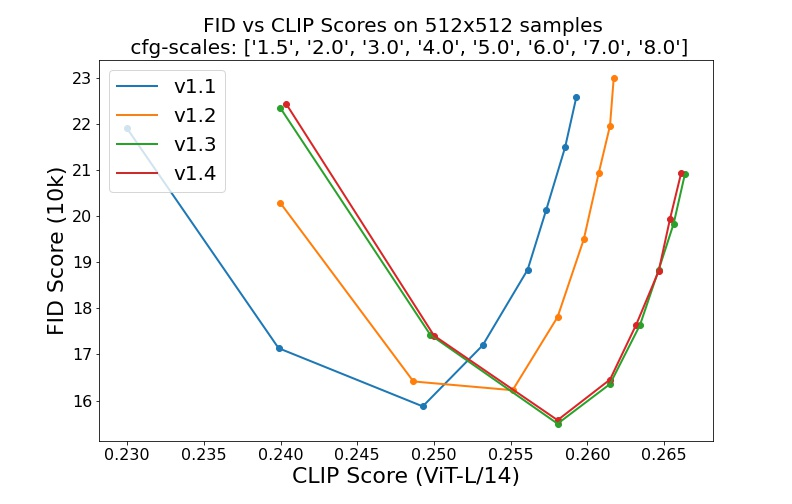
\includegraphics[width=\textwidth]{./images/graph-sdv1.jpg}
        \caption{}
    \end{subfigure}
    \hfill
    \begin{subfigure}[b]{0.49\textwidth}
        \centering
        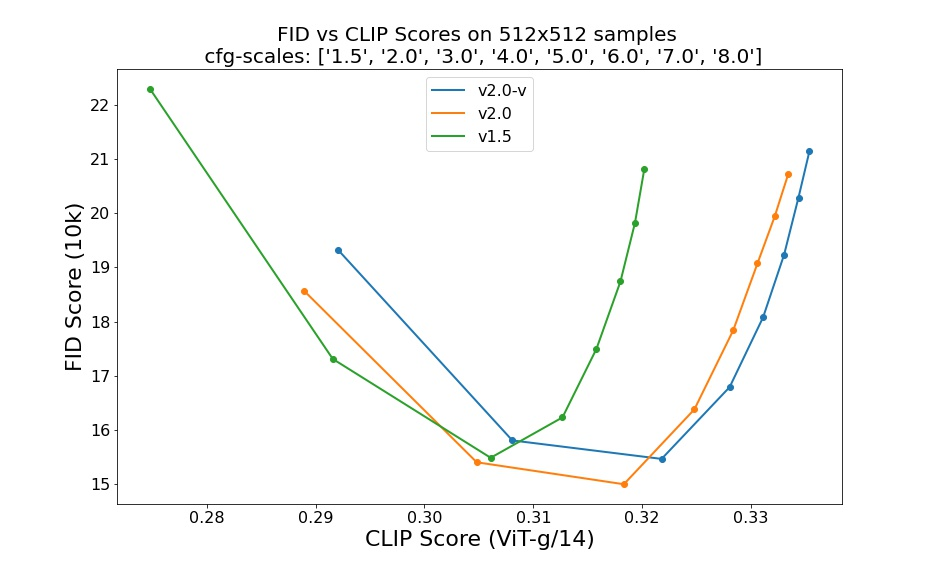
\includegraphics[width=\textwidth]{./images/graph-sdv2.jpg}
        \caption{}
    \end{subfigure}
    \caption{Évaluations avec différentes échelles d'orientation. \cite{rombach2021highresolution}}
    \label{fig:comparaison_sd}
\end{figure}


\subsubsection{Génération d'images}

Une fois notre modèle entrainé, nous pouvons exécuter des inférences pour générer de nouvelles images d'un char Leclerc.
Étant donné que notre jeu de données de véhicules militaires d'origine ne contient pas d'images prises à distance ou dans lesquelles le sujet est partiellement caché, nous avons générer de telles images en redigant des prompts complexes.\\

Ci-dessous nous avons un extrait de script permettant de générer les images:
\begin{lstlisting}[language=Python, basicstyle=\footnotesize\ttfamily, breaklines=true]
    lora_model_id = "../adomvi-dream-tank-xl_1024"
    model_base = "stabilityai/stable-diffusion-xl-base-1.0"
    
    prompts = {
        "desert": "[L] tank moving in the desert behind rocks, seen from the top of a distant hill, respecting realistic scale and dimensions",
        "urban_combat": "[L] tank in urban combat, maneuvering between buildings, seen from a high-rise far away, respecting realistic scale and dimensions",
        "forest_camouflage": "[L] tank camouflaged in a dense forest, barely visible among trees, seen from very far away, respecting realistic scale and dimensions",
    }
    
    negative_prompt = "close-up, upfront, unobstructed, bad scale, inaccurate canons, extra canons, out of frame, lowres, text, error, cropped, worst quality, low quality, jpeg artifacts, duplicate, bad proportions, extra elements, malformed structures"
    
    generate_images(
        lora_model_id=lora_model_id,
        model_base=model_base,
        prompts=prompts,
        negative_prompt=negative_prompt,
        inference_dir=inference_dir,
        width = 1024,
        height = 1024,
        num_inference_steps = 150
    )
\end{lstlisting}

Sur ce schéma, nous présentons une trame de fonctionnement du modèle text2image
\begin{figure}[H]
    \center
    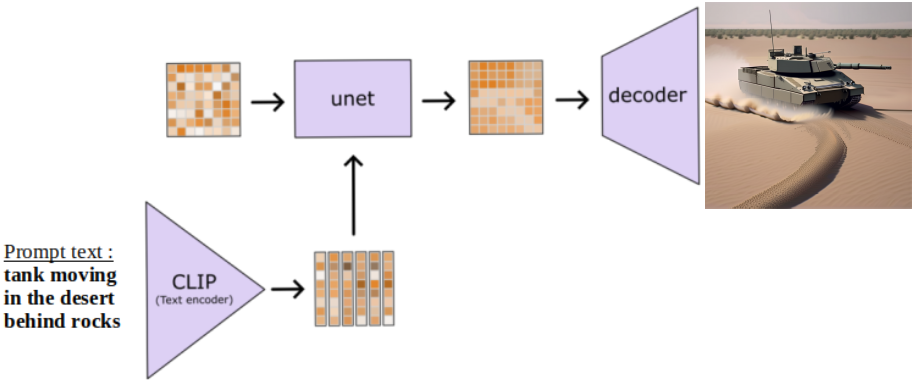
\includegraphics[width=\textwidth]{./images/shema_sd.png}
    \caption{Schéma du fonctionnement normal de Stable Diffusion}
\end{figure}


\subsubsection{Images générées}

Plusieurs modèles de Stable Diffusion ont été utilié durant cette expérience.

\begin{figure}[H]
    \center
    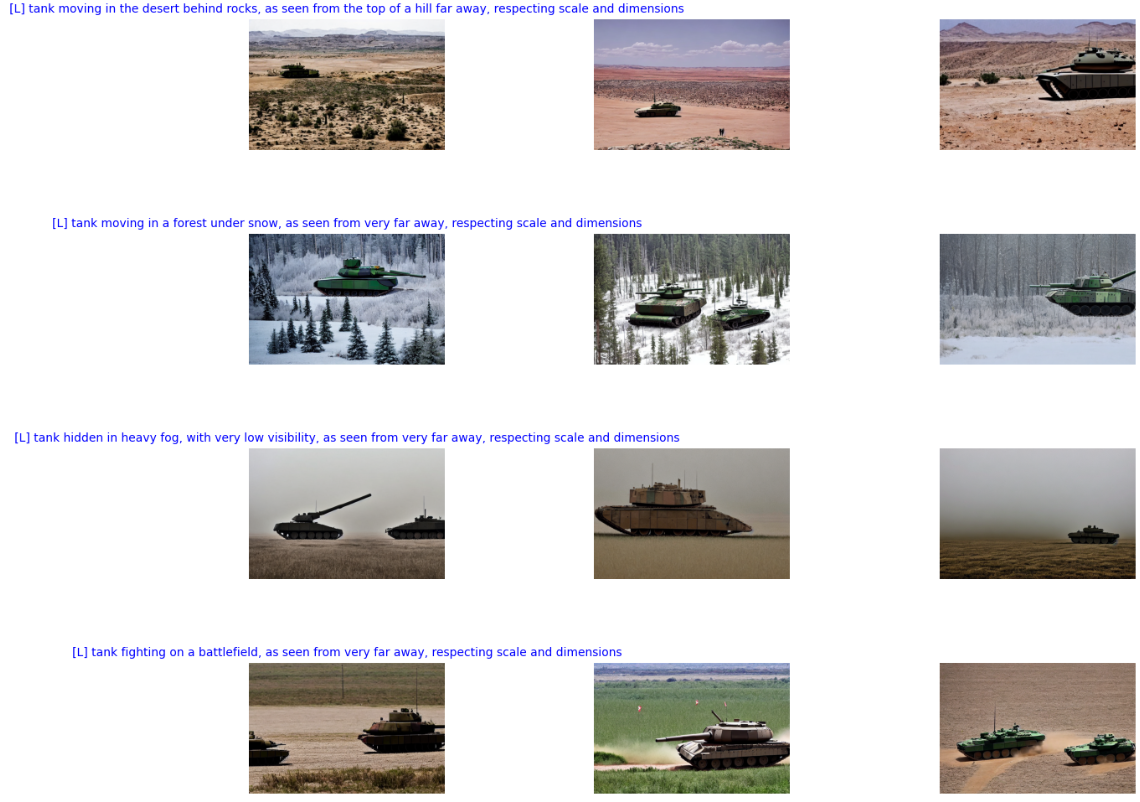
\includegraphics[width=\textwidth]{./images/v1-5_sd_dreambooth.png}
    \caption{prompts + Images générés avec le modèle stable-diffusion v1.5}
    \label{fig:image_sdv15}
\end{figure}

\begin{figure}[H]
    \centering
    \begin{subfigure}[b]{0.49\textwidth}
        \centering
        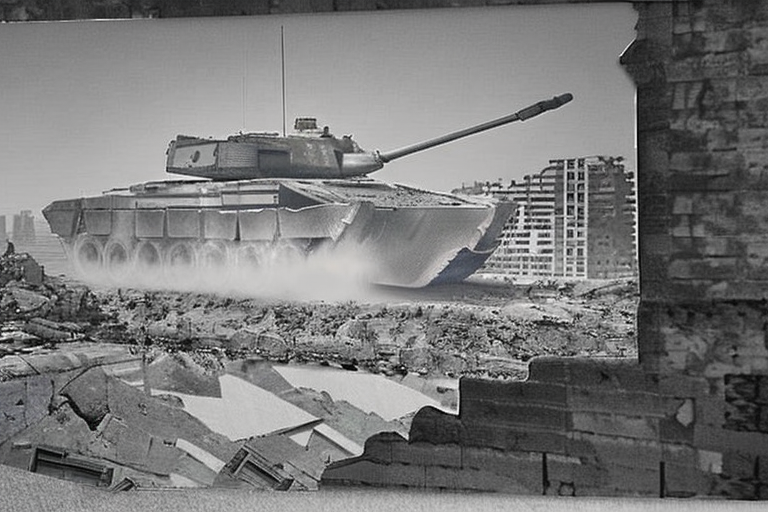
\includegraphics[width=\textwidth]{./images/v2_tank-city_ruins-1.png}
        \caption{Dans les ruines de la ville}
    \end{subfigure}
    \begin{subfigure}[b]{0.49\textwidth}
        \centering
        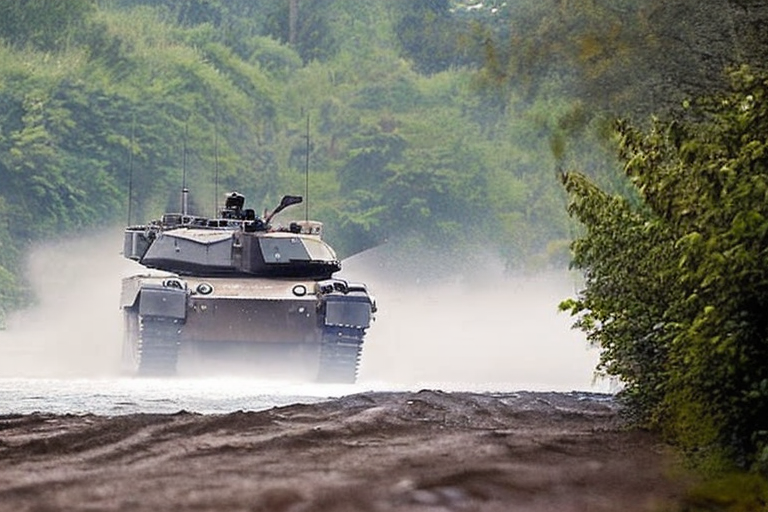
\includegraphics[width=\textwidth]{./images/v2_tank-rainy_day-3.png}
        \caption{Par un jour pluvieux}
    \end{subfigure}
    \hfill
    \begin{subfigure}[b]{0.49\textwidth}
        \centering
        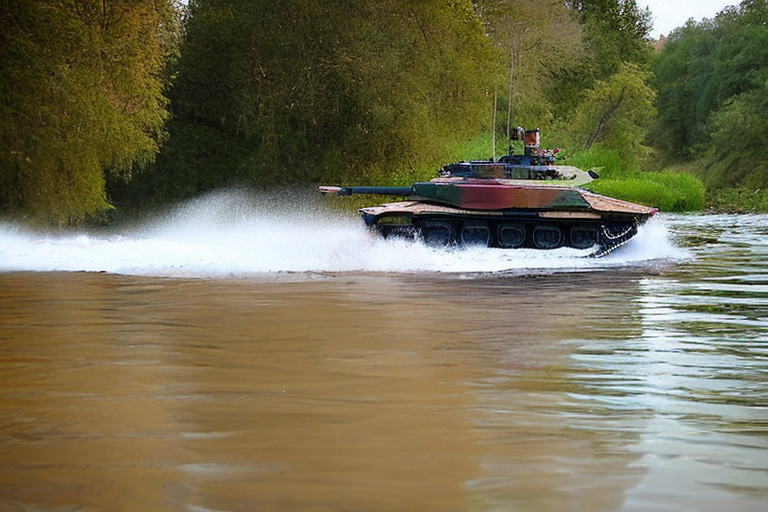
\includegraphics[width=\textwidth]{./images/v2_tank-river_crossing-0.png}
        \caption{Traversée de rivière}
    \end{subfigure}
    \begin{subfigure}[b]{0.49\textwidth}
        \centering
        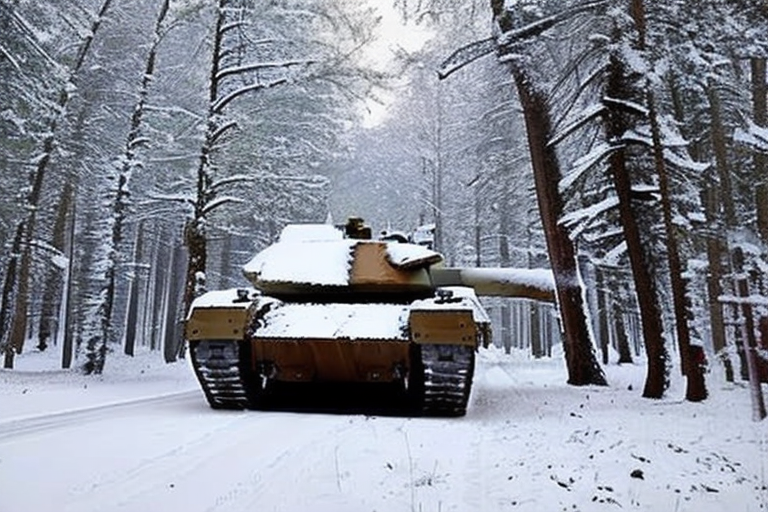
\includegraphics[width=\textwidth]{./images/v2_tank-snow-1.png}
        \caption{Sous la neige}
    \end{subfigure}
    \caption{Images générés avec le modèle stable-diffusion v2}
    \label{fig:image_sdv2}
\end{figure}


\begin{figure}[H]
    \centering
    \begin{subfigure}[b]{0.49\textwidth}
        \centering
        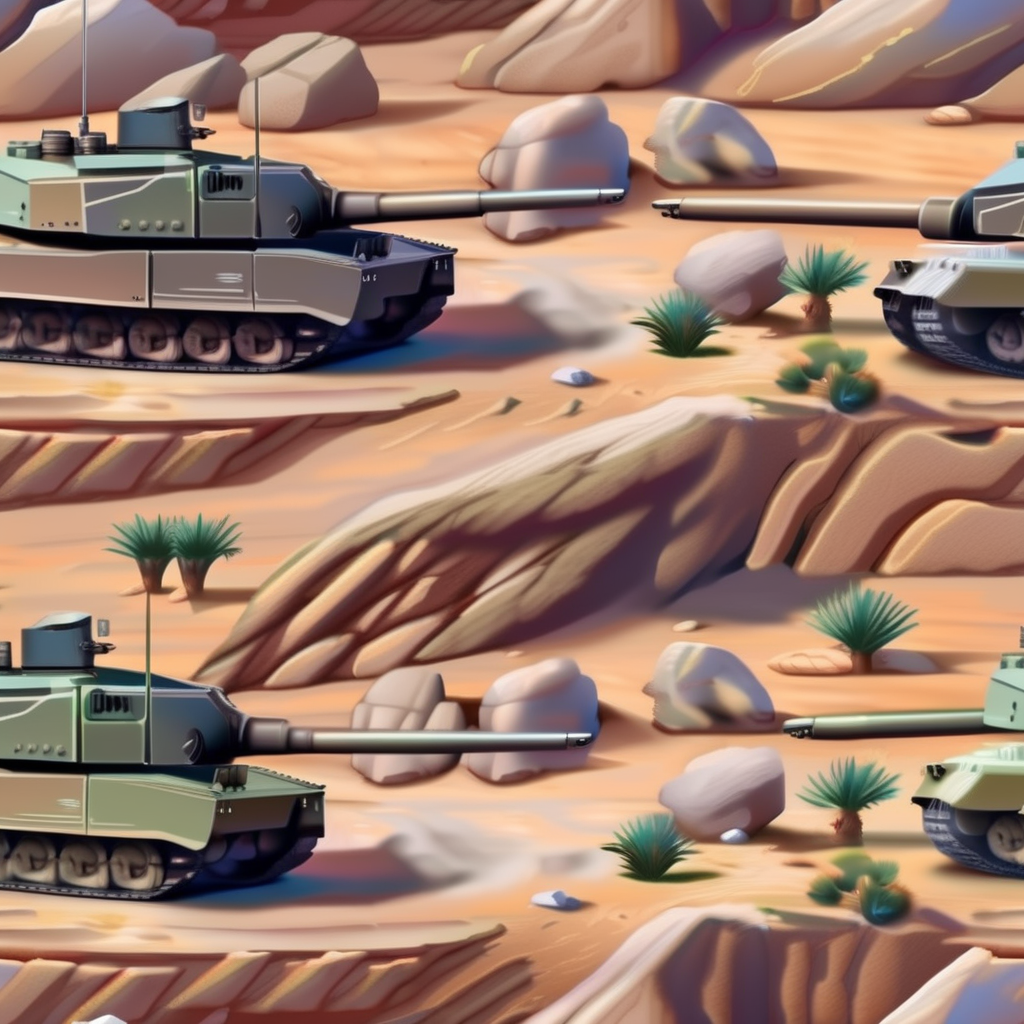
\includegraphics[width=\textwidth]{./images/xl_tank-desert-3.png}
        \caption{Dans le désert}
    \end{subfigure}
    \begin{subfigure}[b]{0.49\textwidth}
        \centering
        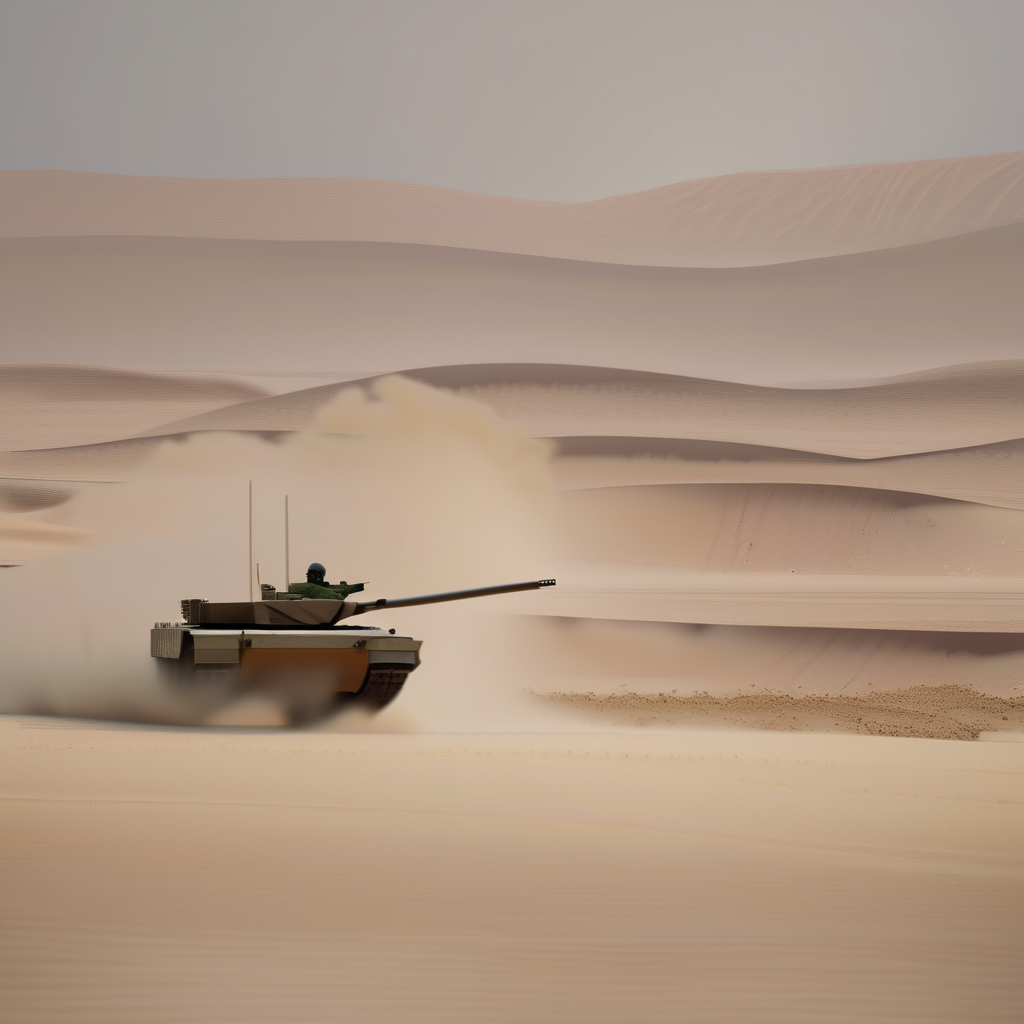
\includegraphics[width=\textwidth]{./images/xl_tank-desert_storm-2.png}
        \caption{Tempête de sable dans le désert}
    \end{subfigure}
    \hfill
    \begin{subfigure}[b]{0.49\textwidth}
        \centering
        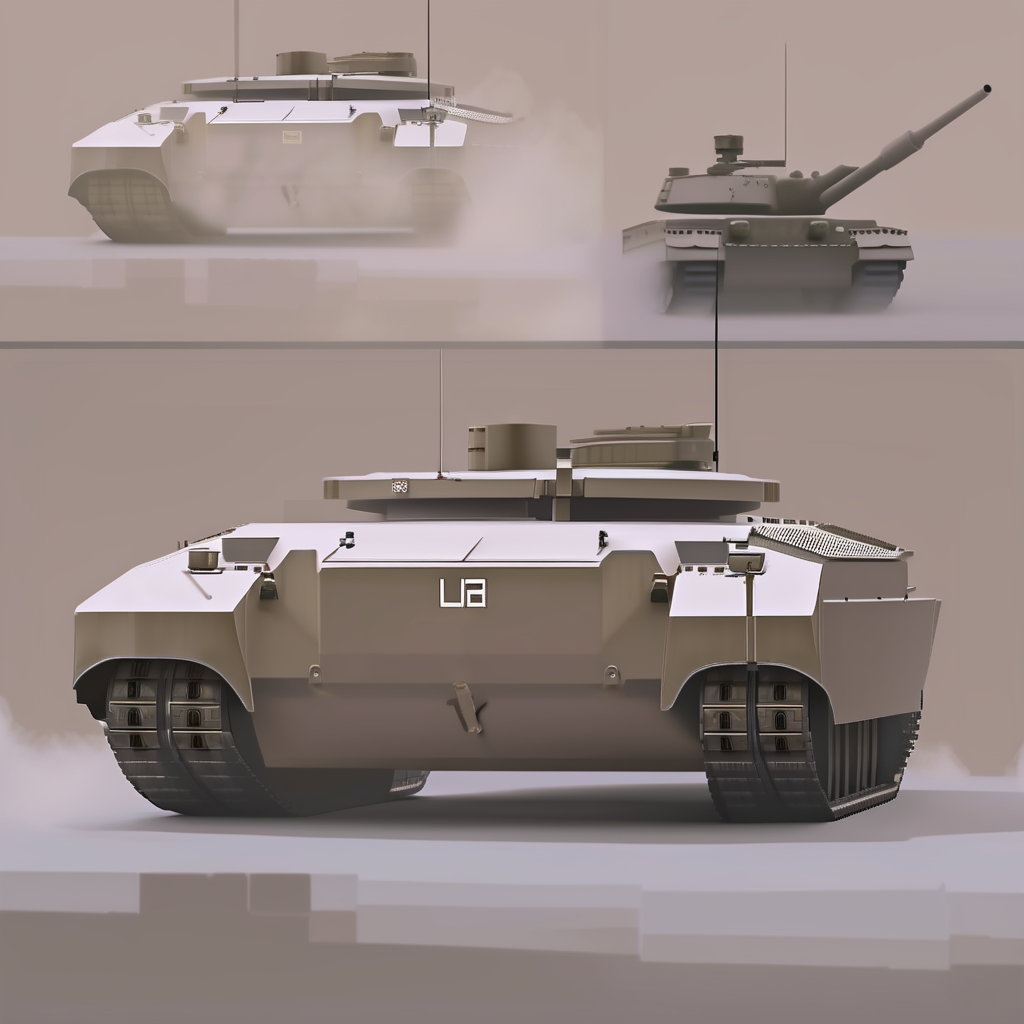
\includegraphics[width=\textwidth]{./images/xl_tank-fog-2.png}
        \caption{Dans le brouillard}
    \end{subfigure}
    \begin{subfigure}[b]{0.49\textwidth}
        \centering
        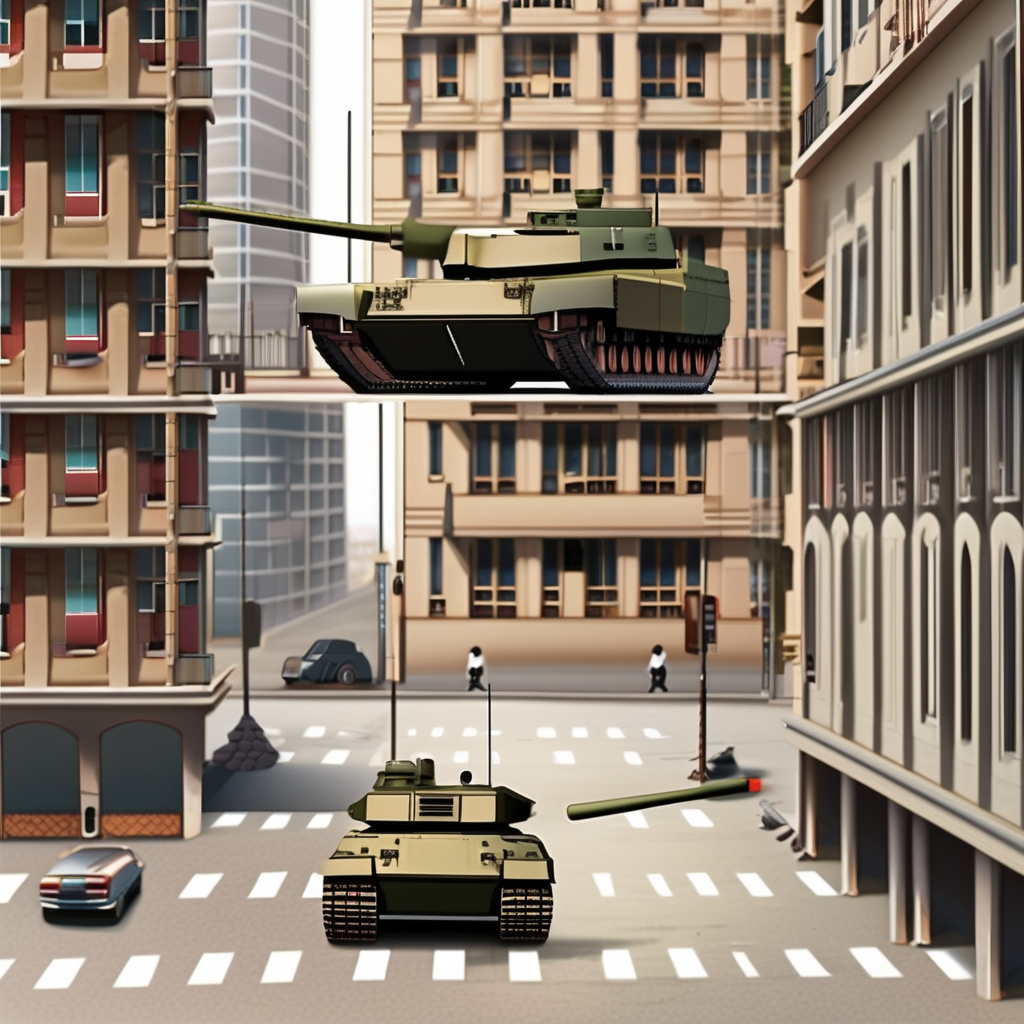
\includegraphics[width=\textwidth]{./images/xl_tank-urban_combat-1.png}
        \caption{Combat urbain}
    \end{subfigure}
    \caption{Images générés avec le modèle stable-diffusion XL}
    \label{fig:image_sdxl}
\end{figure}


Contrairement à la technique de transformation d'images, la génération d'images synthétiques ne fournit pas les anotations des véhicules présents sur les images.
Après la génération des ces images, elles doivent être validés par l'équipe de la DGA TT avant d'être annotées.

Nous continuons les expériences en modifiant les valeurs des hyperparamètres des différents modèles afin d'obtenir des images réalistes et optimales nécessaire à l'entrainement de notre modèle de detection d'objet dans les images.


